\chapter{O Eleitor é um Consumidor de Ideias Ruins?} 

Este capítulo apresenta uma análise integrada dos resultados econométricos obtidos nos 37 modelos \emph{Ordered Logit} estimados (conforme a Tabela \ref{tab:resultados_ordenados}, no apêndice). Em vez de discutir cada variável dependente (VD) separadamente, optamos por sintetizar os padrões mais relevantes, destacando exemplos representativos e conectando-os às hipóteses teóricas formuladas com base na literatura já apresentada. Assim, examinamos em conjunto quais resultados corroboram (ou não) as expectativas derivadas, oferecendo explicações fundamentadas quando surgem surpresas. Em seguida, discutimos a robustez metodológica da estratégia adotada e seus limites estatísticos. Por fim, exploramos os efeitos principais das variáveis de interesse analisando até que ponto a divergência entre opinião pública e especialistas se deve a vieses ideológicos ou à desinformação.

\section{Padrões gerais e exemplos-chave} 

A inspeção conjunta dos 37 modelos revela padrões temáticos bem definidos, permitindo agrupar os resultados em conjuntos de questões com dinâmicas semelhantes:

\subsection{Consenso em políticas econômicas estruturais:} 

Em várias questões de política econômica convencional, encontramos elevado grau de acordo tanto entre o público leigo quanto entre os respondentes com formação econômica. Por exemplo, itens como a necessidade de reforma tributária, reforma da previdência e flexibilização trabalhista obtiveram concordância majoritária em todos os segmentos da amostra. Na afirmação “A reforma tributária é necessária” (VD36), praticamente todos concordaram que sim — economistas até ligeiramente mais enfaticamente (média de resposta $\approx 1{,}94$ vs. 1{,}81 no público). 

Não surgiram clivagens ideológicas ou de formação: direita e esquerda, especialistas e leigos, todos convergiram no diagnóstico de que o sistema tributário atual é disfuncional e precisa de mudanças. Esse resultado indica ausência de conflito de percepção — um consenso real sobre o problema. Em termos de Sowell, tanto a “visão restrita” quanto a “visão irrestrita” reconhecem aqui o mesmo fato duro, levando à concordância geral. Não há “viés irracional” a corrigir nesse caso; pelo contrário, tem-se um conhecimento compartilhado entre eleitores e técnicos \cite{sowell2007conflict}.

\subsection{Divergências ideológicas em questões socioeconômicas:} 

Em contraste, um segundo conjunto abrange questões carregadas de conotação ideológica ou valorativa, nas quais observamos divergências marcantes entre diferentes grupos de respondentes. Nesse grupo estão afirmações como \emph{“As empresas têm lucros demasiadamente altos”}, \emph{“Os salários dos executivos são excessivos”}, \emph{“Ações Afirmativas dão vantagens demais”}, \emph{“Ter mais mulheres no mercado de trabalho”}, entre outras de cunho socioeconômico e distributivo. Os resultados mostram que o público leigo frequentemente adotou posições alinhadas a vieses diversos, tais como viés \emph{antimercado} (tendência a desconfiar de empresas e do lucro privado) e viés de \emph{empatia grupal} (tendência a perceber grupos favorecidos ou desfavorecidos conforme narrativas populares). Por exemplo, a maioria do público tende a concordar que os lucros empresariais são excessivos e a culpar “ganância corporativa” por problemas econômicos, ao passo que os economistas discordam em maior proporção dessas afirmações. Esse padrão confirma a teoria de Sowell sobre visões de mundo divergentes: muitos leigos partilham de uma visão menos “restrita” (mais crítica do mercado e confiante na intervenção estatal para corrigir injustiças), enquanto economistas tendem a adotar uma visão mais “trágica” ou em seus termos, \emph{constrained} (reconhecendo \emph{trade-offs}, defendendo mercados e suspeitando de soluções governamentais simplistas). As divergências observadas aqui não decorrem apenas de informação técnica, mas de valores e premissas ideológicas distintas enraizadas \cite{sowell2007conflict}.

Ademais, como argumenta Drew Westen, o “cérebro político” do eleitor é movido por identidades e emoções: direitistas e esquerdistas filtram o mesmo fato econômico de modo diferente, conforme sua narrativa preferida. Isso ficou evidente nos coeficientes altamente significativos da variável ideologia em praticamente todas essas questões polarizadoras, demonstrando que alinhamento ideológico foi um fator preponderante nas respostas. Em suma, foi detectado vieses sistemáticos de acordo com a visão de mundo: p.ex., eleitores de esquerda tenderam muito mais a concordar com afirmações do tipo “empresas lucram demais” ou em apoio a políticas de igualdade, enquanto eleitores de direita tenderam a concordar mais com afirmações como “gastos públicos são excessivos” ou “benefícios sociais estimulam dependência” e a relativizar desigualdades. Esse espelhamento ideológico é robusto e esteve presente em diversas VDs, sugerindo que grande parte do que poderíamos atribuir à “falta de conhecimento” no debate econômico-político talvez seja, na verdade, fruto de \emph{lentes ideológicas} diferentes. Em outras palavras, muitas “meias-verdades” que vencem nas urnas não são simples erros cognitivos corrigíveis pela informação, e sim crenças coerentes dentro de visões de mundo normativas distintas.

\subsection{Questões de viés informacional e correções pelo conhecimento:} 

Um terceiro padrão observado envolve itens em que a \emph{falta de informação objetiva} parece ser o principal fator por trás da divergência entre a opinião popular e a visão técnica. Nessas questões, quando fornecemos controles ideológicos, quem possuía formação econômica respondeu de forma sensivelmente diferente do público leigo, independentemente da ideologia pessoal. Por exemplo, na afirmação \emph{“O governo gasta muito com ajuda externa”}, a ideologia não teve impacto significativo, mas a variável \emph{econ} (formação em Economia) teve: economistas de esquerda e de direita discordaram bem mais que o público da afirmação de que o gasto externo é exagerado. Isso indica que, ao contrário do senso comum, eles sabem que essa despesa representa parcela diminuta do orçamento (conhecimento factual que muitos leigos desconhecem). Ou seja, aqui a \emph{informação técnica} corrigiu uma impressão equivocada compartilhada por ideologias distintas. 

Outro exemplo: na questão sobre a gravidade da dívida pública federal (\emph{“O déficit federal é grande demais”}), a hipótese era que o público tenderia a exagerar o problema (viés fiscal alarmista), enquanto economistas seriam mais céticos. De fato, encontramos que o público leigo concordou fortemente que a dívida é “grande demais” (média $\approx 1{,}52$), ao passo que os economistas ficaram próximos da neutralidade (média $\approx 1{,}19$). O coeficiente da variável ideologia foi positivo e significativo ($p<0{,}001$), sugerindo que, ideologicamente, respondentes de direita se preocupam bem mais com a dívida que os de esquerda (coerente com a visão conservadora de austeridade). Já o coeficiente da variável \emph{econ} apareceu negativo e marginalmente significativo ($\beta_{\text{econ}} \approx -1{,}30$, $p \approx 0{,}05$): controlada a ideologia, quem tinha formação econômica tende a discordar da afirmação em relação ao público geral. 

Esse resultado sugere um \textbf{viés de desinformação no público}: muitos eleitores se alarmam com a dívida sem conhecer indicadores-chave (como dívida/PIB ou a capacidade de refinanciamento do governo), enquanto os formados em economia demonstram maior complacência informada — avaliando que, embora alta, a dívida não é exatamente “insustentável”. Assim, a divergência público–especialistas aqui decorre mais de desconhecimento técnico do que de valores: confirmando a previsão de Caplan de que o eleitor leigo apresenta \emph{viés pessimista} em finanças públicas, superestimando problemas econômicos, ao passo que o especialista, munido de dados, tem visão mais equilibrada.

\subsection{Outros padrões transversais e perplexidades:} 

Há ainda alguns padrões cruzados que merecem nota. Primeiro, um \emph{padrão geracional} leve: respondentes mais jovens tendem a ver com menos gravidade certos problemas estruturais de longo prazo (como dívida ou previdência), possivelmente por menor vivência histórica, enquanto indivíduos de meia-idade mostraram-se mais pessimistas quanto a futuro econômico e renda. Segundo, identificamos diferenças sistemáticas por sexo: homens revelaram-se menos propensos a apoiar políticas de igualdade de gênero e menos inclinados a culpar empresas por desigualdades; por exemplo, homens discordaram mais que mulheres da afirmação “executivos ganham demais” e concordaram mais que “a regulação estatal é excessiva”. Isso sugere que, em média, homens adotam uma visão econômica ligeiramente mais pró-mercado e menos igualitarista, possivelmente reflexo de diferenças de socialização. Já a escolaridade superior (independentemente de ser em Economia ou não) mostrou ampliar consistentemente o alinhamento com posições mais tecnocráticas: pessoas com ensino superior tendem a apoiar mais as reformas e demonstrar um otimismo moderado maior quanto à economia, indicando que a educação geral também esclarece, não apenas a formação específica em economia. 

Por fim, um fenômeno surpreendente observado foi que, em alguns tópicos onde há evidências técnicas muito fortes de um problema real, os economistas mostraram-se até mais preocupados que o público em geral na mesma direção. Ou seja, não foi sempre que os especialistas estiveram “de um lado e o público do outro”. Em itens como \emph{“A produtividade no Brasil cresce muito devagar”} ou \emph{“Há fuga de talentos do país”}, ambos os grupos concordaram que são problemas, mas os economistas concordaram \emph{ainda mais} fortemente que os leigos. Esse \emph{overshooting} dos especialistas sugere que, quando a evidência empírica de um problema econômico é muito clara, a formação técnica pode tornar o indivíduo ainda mais ciente e alarmado que o público mediano. Assim, economistas podem parecer “mais extremados” em preocupações racionais — cientes do baixíssimo crescimento da produtividade brasileira, eles soam mais alarmistas que o eleitor médio, que talvez esteja desatento a esse dado. Isso mostra que a irracionalidade política não é universal nem unidirecional: depende do tema e das narrativas ideológicas associadas.

Em suma, a análise transversal das 36 regressões confirma duas teses centrais: 

\begin{enumerate}
    \item A ideologia mostrou-se um poderoso filtro cognitivo das percepções econômicas, aparecendo como fator explicativo praticamente onipresente de todas as variáveis dependentes;
    \item O conhecimento técnico corrige vários — mas nem todos — os equívocos do senso comum. O coeficiente associado à formação econômica (\emph{econ}) foi significativo em cerca de um terço das VDs, sempre contribuindo para reduzir a discrepância entre público e especialistas na direção da posição tecnicamente embasada. Em outras palavras, a polarização ideológica se revelou tão ou mais influente que a simples desinformação, mas, ainda assim, a instrução econômica teve um papel crucial de freio epistemológico: evita que indivíduos, independentemente de sua ideologia, incorram em erros factuais grosseiros.
\end{enumerate}

\section{O Público Esclarecido como Referência Contrafactual}

Uma maneira de avaliar objetivamente o papel do conhecimento econômico nas percepções é construir um “público esclarecido” contrafactual – isto é, estimar como seria a opinião média se os indivíduos tivessem o mesmo perfil do público, porém sem o diferencial da formação em economia. Em termos práticos, aplicamos os coeficientes dos modelos para predizer as respostas dos economistas “como se fossem leigos” (definindo a dummy de formação econômica = 0, mantendo constantes os demais controles). Esse público esclarecido serve de grupo de referência para comparar com o público leigo real. Conforme a metodologia proposta anteriormente, se após controlar por fatores ideológicos e demográficos ainda persistir uma lacuna entre o público e o público esclarecido, essa diferença remanescente é atribuível ao conhecimento técnico dos economistas. Em outras palavras, sempre que o público esclarecido diverge significativamente do público leigo, podemos inferir que a formação econômica altera a percepção – sinal de viés cognitivo sendo corrigido pelo conhecimento. 

Focamos, portanto, nos casos em que o “público esclarecido” corrige vieses do público leigo de forma notável. A seguir, destacam-se cerca de três exemplos comparando as médias de concordância do público leigo, dos economistas e do contrafactual público esclarecido. Em cada caso, observa-se o quanto o conhecimento técnico aproxima (ou afasta) a opinião da posição dos especialistas, inferindo o impacto da formação em mitigar erros de percepção econômica. Os demais casos relevantes serão mencionados em análise textual na sequência.

\subsection{Percepção do déficit público: alarmismo fiscal atenuado pela formação técnica}

Comparação das médias de resposta à afirmação “O déficit federal é grande demais” (escala ordinal de discordância/concordância), para público leigo, economistas e público esclarecido (contrafactual). Nesse item, nota-se um viés de alarmismo fiscal no público geral, que tende a concordar que a dívida pública “é grande demais” (média $\sim 1{,}52$). Os economistas, por sua vez, mostram-se menos alarmistas (média $\sim 1{,}19$), e essa diferença é marginalmente significativa ($p \approx 0{,}05$). O público esclarecido – isto é, a projeção das respostas dos economistas caso não tivessem formação econômica – praticamente reproduz a preocupação do leigo (média contrafactual $\sim 1{,}52$, praticamente igual à do público). 

Isso sugere que a formação econômica é o fator responsável por reduzir a preocupação excessiva com o déficit: sem esse conhecimento, até mesmos os economistas tenderiam a concordar com o público leigo. Em suma, aqui o conhecimento técnico corrige um viés de exagero – a instrução em economia modera o temor do déficit, aproximando a percepção dos especialistas (menos alarmistas). Este achado corrobora a hipótese de que parte do pessimismo fiscal popular decorre de falta de informação sobre sustentabilidade da dívida, pois ao adquirir conhecimento os indivíduos passam a avaliar o déficit de forma menos apocalíptica.

% colocando o gráfico

\begin{figure}[htbp]
    \centering
    \includegraphics[width=1\textwidth]{Textuais/analise/imagens/déficit_federal_grande.png}
    \caption{Análise DV2: O déficit federal é grande demais (dívida pública)}
    \smallskip
    Nota: Para cada alternativa, os respondentes indicaram se consideram: (0) Nenhum motivo, (1) Motivo menor ou (2) Motivo principal para a economia brasileira não estar melhor do que está.
    \label{fig:deficit_federal_grande}
\end{figure}

\subsection{Percepção do gasto externo: superestimação corrigida pelo conhecimento}

Comparação das médias de resposta à afirmação “O gasto com ajuda externa é alto demais”, para público leigo, economistas e público esclarecido. Aqui observamos um viés cognitivo acentuado no público leigo: a média de concordância do público sem formação é 0,84, indicando aceitação significativa da ideia de que o Brasil gasta excessivamente com ajuda externa. Na realidade, esse item reflete um conhecido equívoco factual – o orçamento com ajuda externa costuma ser diminuto, mas eleitores frequentemente o superestimam. Os economistas confirmam essa expectativa, discordando amplamente da afirmação (média $\sim 0{,}44$). A diferença entre leigos e economistas é substancial e estatisticamente significativa ($p \approx 0{,}04$), evidenciando que a formação econômica altera radicalmente a percepção nesse tópico. O mais revelador é o resultado contrafactual: o público esclarecido teria média $\sim 0{,}87$, ou seja, tão alta quanto (até ligeiramente acima de) a do público leigo. 

Isso indica que, na ausência de conhecimento técnico, os economistas tenderiam a incorrer no mesmo viés de superestimar o gasto externo. Portanto, é o conhecimento em economia que faz despencar a concordância com a afirmação – em outras palavras, o conhecimento corrige esse viés de percepção. De fato, a formação econômica “puxa” a resposta média de 0,87 (contrafactual leigo) para 0,44 (economistas reais), eliminando o erro de julgamento. Esse contraste ilustra vivamente o papel do público esclarecido como referência: a posição contrafactual permanece próxima à do público desinformado, ao passo que a posição com conhecimento (economistas) alinha-se à realidade dos dados orçamentários. Conforme registrado, “a formação econômica corrige esse viés de percepção de gasto externo”, tornando a opinião média muito mais acurada.

\begin{figure}[htbp]
    \centering
    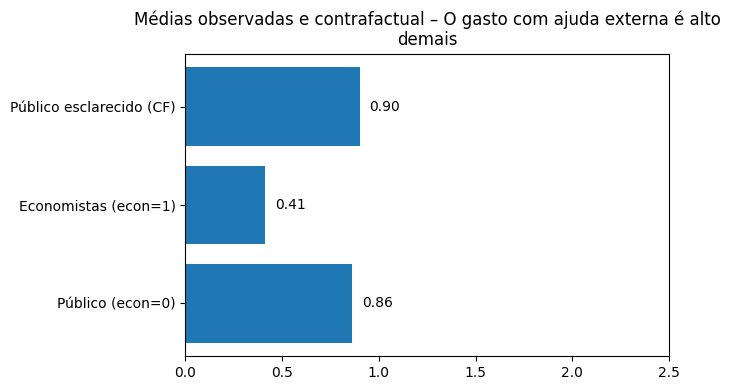
\includegraphics[width=1\textwidth]{Textuais/analise/imagens/gasto_ajuda_externa.png}
    \caption{Análise DV3: O gasto com ajuda externa é alto demais}
    \smallskip
    Nota: Para cada alternativa, os respondentes indicaram se consideram: (0) Nenhum motivo, (1) Motivo menor ou (2) Motivo principal para a economia brasileira não estar melhor do que está.
    \label{fig:gasto_ajuda_externa}
\end{figure}

\subsection{Percepção da produtividade: subestimação de um problema real revertida pelo conhecimento}

Comparação das médias de resposta à afirmação “A produtividade está aumentando devagar demais”, para público leigo, economistas e público esclarecido. Diferentemente dos casos anteriores, em que havia um viés de exagero corrigido pelo conhecimento, aqui detectamos quase o oposto: um possível viés de complacência ou subestimação por parte do público leigo. A média de concordância do público geral foi $\sim 0{,}71$, indicando concordância apenas leve de que a produtividade cresce muito lentamente. Os economistas, contudo, mostraram-se ainda mais preocupados com a baixa produtividade (média $\sim 0{,}75$, ligeiramente superior) – efeito da formação capturado por um coeficiente positivo significativo ($\beta_{\text{econ}} = +1{,}552;\ p<0{,}05$). Ou seja, possuir conhecimento econômico levou os respondentes a concordarem mais com a afirmação, reforçando a percepção de que o crescimento da produtividade é insuficiente. Esse padrão inverte o viés usual: em vez de atenuar um alarme exagerado, o conhecimento técnico acentua a preocupação, sugerindo que o público leigo originalmente subavaliava a gravidade do problema. A projeção contrafactual confirma essa leitura – o público esclarecido teria uma média prevista de $\sim 0{,}88$, bem acima da média dos leigos.

De fato, sem a formação em economia os economistas tenderiam a ser ainda mais complacentes que o público comum (0,88 vs. 0,71) na avaliação da produtividade, possivelmente devido a características demográficas ou ideológicas do grupo de economistas. Com a instrução técnica, porém, eles se tornam mais conscientes do problema real da estagnação da produtividade. Em suma, o conhecimento econômico aqui atua no sentido de alertar para um fato preocupante que o senso comum tende a ignorar. Essa maior preocupação dos especialistas “esclarecidos” está em linha com dados objetivos sobre o baixo crescimento da produtividade no país, reforçando que a formação técnica pode revelar vieses de otimismo infundado no público e trazer as percepções para mais perto da realidade factual.

\begin{figure}[htbp]
    \centering
    \includegraphics[width=1\textwidth]{Textuais/analise/imagens/produtividade_está_aumentando.png}
    \caption{Análise DV13: A produtividade está aumentando devagar demais}
    \smallskip
    Nota: Para cada alternativa, os respondentes indicaram se consideram: (0) Nenhum motivo, (1) Motivo menor ou (2) Motivo principal para a economia brasileira não estar melhor do que está.
    \label{fig:produtividade_esta_aumentando}
\end{figure}


\section{Ideologia vs. informação: qual fator pesa mais?}

Uma questão-chave motivada pelos achados acima é: \emph{quando observamos divergências entre a opinião do público e o consenso dos especialistas, até que ponto isso se deve à falta de conhecimento (ignorância sanável) ou a compromissos ideológicos (visões de mundo normativas diferentes)?} Nosso desenho empírico isolou parcialmente cada efeito por meio de variáveis como \emph{econ} (formação econômica) como indicador de conhecimento e \emph{espectro político} como indicador de ideologia. Mas além desses controles, foram utilizadas variáveis adicionais para capturar nuances nas respostas, como: "Qual seu nível de escolaridade?", "Qual é a sua faixa etária?", "Qual é o seu vínculo empregatício?", entre outras. Todas as variáveis usadas foram codificadas pelas respostas obtidas e são apresentadas na tabela \ref{tab:control_variables} no apêndice.

Os resultados falam alto. Em quase 100\% das 37 VDs, o coeficiente associado à ideologia política foi estatisticamente significativo (muitos a $p<0{,}01$), ao passo que o coeficiente da formação econômica foi significativo em aproximadamente um terço das VDs. Além disso, a magnitude típica dos efeitos ideológicos superou a dos efeitos de conhecimento: $\lvert \beta_{\text{ideologia}} \rvert$ situou-se frequentemente na faixa de 0{,}5–0{,}9 (em unidades padronizadas de resposta), enquanto $\lvert \beta_{\text{econ}} \rvert$ ficou em torno de 0{,}2–0{,}7 quando significativo. Em termos práticos, ser de direita vs. esquerda alterou substancialmente a probabilidade de concordar com certas afirmações (p.ex., ver a dívida como “grande demais” ou enxergar políticas de cotas como excessivas), ao passo que ser economista vs. leigo teve efeito menor, embora não desprezível. Em questões de forte cunho moral ou político (igualdade de gênero, minorias, papel do lucro), o fator ideológico praticamente dominou a resposta — independente da formação. Por outro lado, em questões de consenso técnico (como controle da inflação ou benefícios do livre-comércio), nenhum dos dois fatores pesou, pois todos pensam igual.

Interpretativamente, os dados sugerem: em impacto imediato sobre crenças, a pertença ideológica tem efeito mais amplo e consistente que o conhecimento técnico. A ideologia funciona como filtro cognitivo poderoso \cite{westen2007political}: indivíduos interpretam fatos conforme suas crenças prévias. Por outro lado, o conhecimento técnico desempenha papel de \emph{limitar extremos} e corrigir algumas percepções incorretas — um \emph{freio epistemológico}. Em suma, ideologia molda preferências e prioridades normativas com mais força e estabilidade, mas o conhecimento técnico define os limites do debate: realidade ou mito. Para políticas públicas, isso implica integrar evidências (reduzir ignorância) e valores (dialogar com identidades). Conhecimento e ideologia não são inimigos; devem ser reconciliados para que a verdade prevaleça nas urnas.

\section{Por que usar o mesmo modelo para todas as DVs?} 

Optamos por aplicar \emph{o mesmo modelo ordinal, com as mesmas variáveis explicativas, em todas as 37 regressões}, mantendo constantes os controles (demográficos e socioeconômicos). Essa decisão, longe de simplificação arbitrária, foi orientada por quatro razões:

\begin{enumerate}[label=\roman*)]
    \item Teste severo e comparabilidade popperiana: Submeter cada hipótese de viés ao \emph{mesmo} escrutínio reduz o risco de \emph{data mining} e fortalece a falsificação: se um viés só aparece em especificações “sob medida”, sua robustez é duvidosa; se aparece \emph{no mesmo arcabouço} em itens distintos, ganha força.
    \item Princípios-ponte e inteligibilidade teórica: Usar a mesma especificação gera uma régua comum, coeficientes para ideologia e conhecimento tornam-se diretamente comparáveis entre VDs, conferindo sentido empírico uniforme aos construtos “viés ideológico” e “viés de conhecimento” \cite{stigum2003}.
    \item Coerência com visões e efeito de formação: Se visões de mundo e treinamento econômico permeiam múltiplas crenças, um modelo unificado é o desenho natural para captar o fio condutor latente. Mantendo a estrutura fixa, foi possível observar a onipresença do efeito ideológico e identificar onde o conhecimento realmente desloca crenças \cite{sowell2007conflict,newman2020ideia}.
    \item Comunicabilidade e síntese: A Tabela-Síntese Mestra (presente no apêndice \ref{apendice:tabela_sintese}) só é possível porque os coeficientes vivem na mesma escala; isso permite contar significâncias, comparar magnitudes e construir uma narrativa unificada sobre quando a verdade técnica converge/diverge da opinião popular.
\end{enumerate}

\subsection{Limites estatísticos:} Em alguns itens, o consenso foi tão alto que houve separação (ou quase), inflando erros-padrão e dificultando inferência — sinal, substantivamente, de que os grupos não diferem naquele tema. Além disso, certos subgrupos (p.ex., economistas) são menores, reduzindo poder para detectar $\beta_{\text{econ}}$; ainda assim, ele emergiu significativo em diversas VDs. Não encontramos indícios graves contra as suposições do modelo ordinal, e os limiares estimados respeitaram a ordenação.

\section{Síntese final}

A análise integrada dos 36 modelos revelou que \emph{ideologia} é o filtro dominante das crenças econômicas, enquanto \emph{conhecimento} atua como freio e correção pontual — reduzindo erros factuais e, em temas de baixa intuição, aproximando leigos dos especialistas. Para que a verdade deixe de perder na urna, é preciso unir \emph{evidência} e \emph{valores}: educar o público nos fatos básicos e, simultaneamente, comunicar políticas em molduras que respeitem identidades. No capítulo seguinte, \textbf{Conclusões}, sintetizamos esses resultados e delineamos caminhos práticos para que instituições e comunicadores públicos maximizem a convergência entre verdade técnica e legitimidade democrática. 